\chapter{ Anwendung von CP in der Scheduling Theorie}

In diesem Kapitel betrachten wir das Formulieren und Lösen einiger Probleme der Scheduling Theorie mit Constraint Programmierung.

Bevor möchten wir die wichtigste Eingenschaften von CP auflisten, die den Ansatz von CP zum Lösen der Scheduling-Probleme besonders attraktiv machen:
\begin{itemize} \itemsep0pt
	\item CP ist besonders für ganzzahlige Variable geeignet. Die Reduktionsmethoden funktionieren auch am besten für endliche Definitionsbereiche der Variablen.
	\item CP passt am besten zum Lösen von Problemen mit vielen Nebenbedingungen
	\item CP ist mehr effektive in den Fällen vieler Nebenbedingungen mit weniger Variablen in jeder einziger Constraint.
	\item Der Ansatz von CP lohnt sich besonders für die Probleme, die sich als eine optimale Abbildung einer geordneten Menge in andere darstellen lassen.
\end{itemize}


\section{Minimieren der gewichteten Gesamtverspätung}
Wir betrachten den Fall eines Schedule mit einer Maschine und der Aufgabe die gewichtete Gesamtverspätung zu minimieren. In $\alpha|\beta|\gamma$ Notation aus \cite{Pinedo} wird dieses Problem als $1||\sum{w_jT_j}$ bezeichnet.

Obwohl die Problemstellung sich einfach formulieren lässt, ist es ein bekanntes $NP$-hartes Problem. Es gibt einen Lösungsansatz mittels Dynamischer Programmierung, der einen pseudopolynomialen Algorithmus liefert \citep[vgl.][]{Pinedo}.

%In CP kann das Problem auf verschiedene Weise formuliert werden. Siehe z.B. Abbildung \ref{fig:WeigtedTardiness}.
%\begin{figure}[h]
%	\centering
%	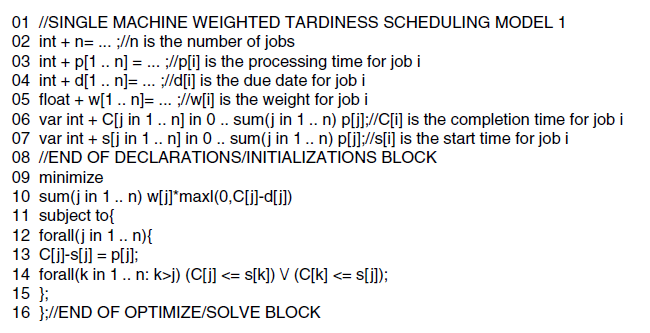
\includegraphics[scale=0.6]{fig/wegntedTardiness.png}
%	\caption{CP-Modell zur Lösung $1||\sum{w_jT_j}$ mittels \cite{OPL}}
%	\label{fig:WeigtedTardiness}
%\end{figure}
%
%\FloatBarrier
%
%In den Zeilen $2-5$ werden die Jobsnummer, Bearbeitungszeiten $p_j$, Sollfertigstellungszeiten $d_j$ und die Gewichte $w_j$ von den Jobs definiert \footnote{$+$ nach dem Typ steht für nicht negative Zahlen.}. Die Variablen des Models sind Startzeiten $r_j$ und Fertigstellungszeiten $C_j$ (Zeile $6$ und $7$).
%Die Zielfunktion des Problems ist $\min \sum{w_jT_j} $, wobei $T_j=\max(0, C_j-d_j)$ ist. Die offensichtliche Nebenbedingungen lauten $C_j=s_j+p_j$ (Zeile $
%13$) und dass kein Job bearbeitet werden kann, bevor die Bearbeitung eines anderes Jobs nicht fertig ist (Zeile $14$).


Einfachste Formulierung des Problems in CP benötigt $n$ Variablen $s_j$ mit dem Definitionsbereich $[0\dots \sum_{j=1..n}p_j]$ für Startzeiten und $n$ Variablen $C_j$ mit dem Definitionsbereich $[0\dots \sum_{j=1..n}p_j]$ für die Fertigstellungszeiten von Jobs . Die Zielfunktion zusammen mit der Nebenbedingungen lassen sie wie folgt ausdrücken:
\begin{align}
 \min & \sum_{j}{w_jT_j} \nonumber \\
 s.t.\quad C_j & = p_j + s_j\qquad\qquad \forall j=1..n \nonumber \\
 C_j  & \le s_k \vee  C_k \le s_j \qquad \forall j,k=1..n,\ k>j \nonumber
\end{align}

In dieser Formulierung sind insgesamt $2n$ Variablen und $\frac{n(n+1)}{2}$ Nebenbedingungen definiert.

Eine andere Formulierung ist möglich, indem man $n$ Variablen $s$ durch $n$ Variablen $pos$ ersetzt, wobei $pos[j]$ die Position des Jobs $j$ in der Bearbeitungsreihenfolge ist. Die Definitionsbereich von $pos$ ist offensichtlich $[1..n]$. Die Nebenbedingungen für diese Formulierung lauten:
\begin{align}
 pos_j & \not= pos_k\qquad\qquad \forall j,k=1..n,\ k>j \nonumber \\
 pos_j  & > pos_k \Leftrightarrow  C_j \ge C_k + p_j \qquad \forall j,k=1..n,\ k\not=j \nonumber \\
 pos_j  & = 1 \Rightarrow C_j=p_j \qquad \forall j=1..n \nonumber
\end{align}

Diese Formulierung enthält  $\frac{3n^2-n}{2}$ Nebenbedingungen, aber ihre Optimierung ist viel langsamer, als vom ersten Modell. Eine mögliche Verbesserung wäre das Hinzufügen von zusätzlichen Nebenbedingungen, die aus der folgende Überlegung entstehen. Wird ein Job auf der Position $j$ platziert, ist die untere Schranke seiner Fertigstellungszeit gleich der Summer seiner Bearbeitungszeit und der Summe $p_i$ von $j-1$ Jobs mit den kleinsten Bearbeitungszeiten. Das bedeutet\footnote{Jobs sind in aufsteigender Reihenfolge der Bearbeitungszeiten geordnet}:
\begin{align}
  pos_j=k \wedge j<=k  & \Rightarrow C_j \ge \sum_{l<=k} p_l \nonumber \\
  pos_j=k \wedge j>k  & \Rightarrow C_j \ge p_j+\sum_{l<k} p_l \nonumber 
\end{align}

Um die Lösung von einem Problem zusätzlich zu beschleunigen, können verschiedene heuristische Verfahren an den Suchverfahren angewendet werden. Für das betrachtete Problem kann man z.B Heuristik WMDD (\glqq {\it weighted modified due date} \grqq)  \citep[siehe][]{WMDD} benutzen.

\section{Job Shop Scheduling}

Eine häufig vorkommende Aufgabe in Scheduling-Theorie ist die Zuordnung von $n$ Jobs zu $m$ Maschinen. Jeder Job besteht dabei aus einer Menge von Operationen $O_j$, die in einer bestimmten Reihenfolge abgearbeitet werden müssen. Typische Bedingungen sind, dass jede Maschine zu jedem Zeitpunkt nur eine Operation bearbeiten kann und umgekehrt dass jede Operation zu jedem Zeitpunkt nur auf einer Maschine abgearbeitet wird. Das Problem mit der Zielfunktion $C_{max}$ (Minimierung des Makespan) wird in Notation aus \cite{Pinedo} als $Jm||C_{max}$ bezeichnet.

Zur Modellierung dieses Problems verwendet man so genannten {\it disjunktiven Graphen} und zur Lösung das {\it Branch \& Bound} Verfahren. Wir betrachten den Ansatz von CP zur Lösung von beschriebenen Job Shop Problem \citep[vgl.][]{CSP}.

Wir definieren Variable $s_o$ für die Startzeit der Operation $o\in O_j$. Offensichtlich gilt $s_o\in \{0,1,\dots C\}$, wobei $C$ eine obere Schranke für $C_{max}$ ist. Man kann aber die Definitionsreich von diesen Variablen ein bisschen einschränken, wenn man den Vorgänger $pred(o)$ und den Nachfolger $succ(o)$ von einer Operation $o$ betrachtet. Dann liegen $s_o$ in $[\sum_{o'\in pred(o)}p_{o'}\dots\ C-p_o-\sum_{o'\in succ(o)}p_{o'}]$.

Die Nebenbedingungen lassen sich wie folgt definieren:
\begin{align}
  s_o + p_o \le s_{o'} &\qquad  o,o'\in O_j,\ o'\in succ(o),\ j=1\dots n \nonumber \\
  s_o + p_o \le C &\qquad  o\in O \nonumber \\
  s_o + p_o \le s_{o'}\ \vee\ s_{o'} + p_{o'} \le s_{o} &\qquad o,o'\in O, o\not=o', m_o=m_{o'} \nonumber 
\end{align}

wobei $O$ die Menge aller Operationen bezeichnet.
Die erste Nebenbedingung garantiert, dass die Operationen auf einen Job sich nicht unterbrechen lassen. In zweiter Nebenbedingung wird sicher gestellt, dass $C$ eine obere Schranke an den Makespan ist. Und die dritte Nebenbedingung besagt, dass unter zwei Operationen $o$ und $o'$, die auf gleicher Maschine abgearbeitet werden, eine vor der anderen abgearbeitet wird oder umgekehrt.

Wie kann man die Bedingungsfortpflanzung für dieses Modell effektiv durchführen? Eine Möglichkeit wurde in der Arbeit von \cite{Nuijten} vorgeschlagen. Für jede Operation $o$ definiert man die frühst möglichste Startzeit $est(o)$ und spät möglichste Startzeit $lst(o)$. Die Werte von $est(o)$ und $lst(o)$ sind entsprechend die kleinste und die größte Werte aus der Definitionsbereich von $s_o$.

Aus der ersten Nebenbedingung folgt, dass $s_o+p_0\le lst(o')$ und $est(o)+p_o\le p_{o'}$ gilt. Deswegen werden die Werte größer als $lst(o')-p_o$ und kleiner als  $est(o)+p_o$ aus der Definitionsbereichen von $s_o$ und $s_{o'}$ entsprechend  entfernt.

Aus der dritten Nebenbedingung folgt $s_o\le lst(o') - p_o$, falls Operation $o$ vor der Operation $o'$ auf einer Maschine abgearbeitet wird, oder $s_o \ge est(o') + p_{o'}$, falls umgekehrt. Wenn es $lst(o') - p_o + 1 \le est(o') + p_{o'} -1$ gilt, dann können alle Werte aus $[lst(o') - p_o + 1 \dots est(o') + p_{o'} -1]$ aus dem Definitionsbereich von $s_o$ gelöscht werden.



\section{Timetabling}

Wir betrachten ein Beispiel der Erstellung eines Zeitplanes (engl. Timetable) mit Hilfe von Constraint Programmierung. Das Beispiel stammt aus der Artikel von \cite{Timetabling} und beschreibt Scheduling eines Rundenturniers für Basketball-Spiele.

Bevor \cite{Timetabling} war die Aufgabe mittels ganzzahliger Programmierung und erschöpfender Suche \citep[siehe][]{Timetabling_Trick} gelöst und die Lösung hat $24$ Stunden gedauert. Im Gegensatz dazu hat die Lösung mit Hilfe von CP weniger als eine Minute gebraucht.

Es wurden $n=9$ Teams betrachtet, für die $2n=18$ Termine festgelegt sollte, sodass an jedem Termin $n-1$ Teams spielen und ein Team nicht spielt (d.h. hat \glqq bye\grqq). Alle Termine sollten in neuen Wochen (von 31.12.1997 bis 1.03.1998) mit einem Wochenende und einen Arbeitstag pro Woche geplant werden.

Das Problem wird in drei Phasen gelöst: \begin{itemize}
\setlength{\itemsep}{0pt}
\item Generierung von einem Muster (engl. pattern) für jedes Team, das für jeden Termin feststellt, ob Team ein Heim-, Auswärtsspiel oder \glqq bye\grqq\ spielen kann. Die Generierung von Mustern hängt von allen formulierten Bedingungen an die Spiele ab. 
\item Suche nach einer Menge von $9$ Mustern, die die Erstellung eines Zeitplanes ermöglichen.
\item Generierung einem Zeitplan, indem man anhand der Menge von Mustern die Zuordnung von Spielen zu den Teams und Paare von Gegner bestimmt.
\end{itemize}

\subsection{Berechnung von Mustern}
\label{Phase2}
Man definiert drei Gruppen von binären Variablen $h_j, a_j, b_j, j=1\dots 18,$ für Heimspiele, Auswärtsspiele und byes und löst das Problem mit Hilfe von Constraint Programmierung. Einige von betrachteten Bedingungen sind:
\begin{itemize}
\setlength{\itemsep}{0pt}

\item jedes Team hat nur ein Spiel an jedem Termin: $h_j+a_j+b_j = 1$

\item s.g. Mirroring: Termine sind paarweise in die vorgegebene Menge $m$ gruppiert, jedes Paar bezeichnet Spiele der gleichen Team: $h_j=a_{j'},\ a_j=h_{j'},\ b_j=b_{j'}\ (j, j')\in m$

\item zwei letzte Spielen können nicht beide Auswärtsspiele sein : $a_{17}+a_{18} = 2$


\item Es sind nicht mehr als zwei Auswärtsspiele nacheinander erlaubt:\\ $a_j+a_{j+1}+a_{j+2}<3$ 

\item Es sind nicht mehr als zwei Heimspiele nacheinander erlaubt:\\ $h_{j}+h_{j+1}+h_{j+2}<3$ 

\item Es sind nicht mehr als drei Auswärtsspiele oder byes  nacheinander erlaubt: \\
$a_j+b_j+a_{j+1}+b_{j+1}+a_{j+2}+b_{j+2}+a_{j+3}+b_{j+3}<4$ 

\item Es sind nicht mehr als vier Heimspiele oder bayes nacheinander erlaubt:\\
$h_j+b_j+h_{j+1}+b_{j+1}+h_{j+2}+b_{j+2} +h_{j+3} ++b_{j+3} +h_{j+4}+b_{j+4} <5 $ 

\item An allen Wochenenden spielt jedes Team vier Heim-, vier Auswärtsspiele und ein bye:   $\sum_{j\in\{2,4,\dots 18\}}h_j = 4$, $\sum_{j\in\{2,4,\dots 18\}}a_j = 4$, $\sum_{j\in\{2,4,\dots 18\}}b_j = 1$

\item Jedes Team spielt Heimspiels oder byes mindestens an zwei von fünf ersten Wochenende $\sum_{j\in\{2,4,6,8,10\}}(h_j+b_j) \ge 2$

\end{itemize}

Die effektivste Suchstrategie in diesem Fall ist Durchzählen von möglichen Werten vom $h,a,b$ in der Reihenfolge $h_1,a_1,b_1,h_2,a_2\dots$.

\subsection{Menge von Mustern}

Es wurden insgesamt $38$ Mustern für das betrachtete Problem gefunden, die in drei $38\times 9$ Matrizen $h,a$ und $b$ gespeichert sind. Das Ziel ist eine Menge aus $9$ Mustern zu finden, die es erlaubt einen zulässigen Zeitplan zu bilden.

Um diese Aufgabe lösen zu können definieren wir binären Variablen $x_i$, $i=1\dots 38$. $x_i=1$, falls das Muster $i$ in die gesuchte Menge kommt, sonst $0$.
Das Modell als formuliert als CSP lautet:
\begin{align}
  \sum_{i}x_i=9 &  \nonumber \\
  \sum_{i}h_{ij}x_i = 4,\ \sum_{i}s_{ij}x_i = 4,\ \sum_{i}b_{ij}x_i = 1 &\qquad  j=1\dots 18 \nonumber \\
  x_i+x_{i'} <1  &\qquad  j=1\dots 18,\ i,i'=1\dots 9,\ i\not=i', \nonumber\\
  & (h_{ij}=0 \vee a_{i'j}=0)\wedge(a_{ij}=0 \vee h_{i'j}=0) \nonumber  
\end{align}

wobei in der dritten Bedingung werden die Muster, die keinen zulässigen Spielplan bilden können, extra ausgeschlossen.

\subsection{Erstellung von einem zulässigen Zeitplan}
Es gibt mehrere Verfahren, um einen zulässigen Zeitplan aus der gegebenen Menge von Mustern zu erstellen. Das Verfahren, das in beschriebenen Artikel verwendet wurde, ordnet erst jedes Team zu einem von $9$ vorhandenen Mustern zu und danach sucht für jedes Team nach den möglichen Gegnern an jedem Termin.

Die Aufgabe der Erstellung eines zulässigen Zeitplanes wird wiederum als ein CP Modell formuliert, das jeweils für jedes Team und jeden Termin einen Gegnern und Spielart (Heim-/Auswärtsspiel oder bye) berechnet. Die Nebenbedingungen werden von allgemeinen Bedingungen an ein Rundenturnier und Bedingungen aus den Abschnitt \ref{Phase2} bestimmt.